\documentclass[tikz,border=2pt]{standalone}
\usepackage{amsmath}
\usepackage{tikz}
\usetikzlibrary{arrows.meta,positioning}

\begin{document}
% y = g(f(x)) changes through the intermediate variable u = f(x): a small change dx becomes
% du = f'(x) dx, which becomes dy = g'(u) du; the rates multiply.
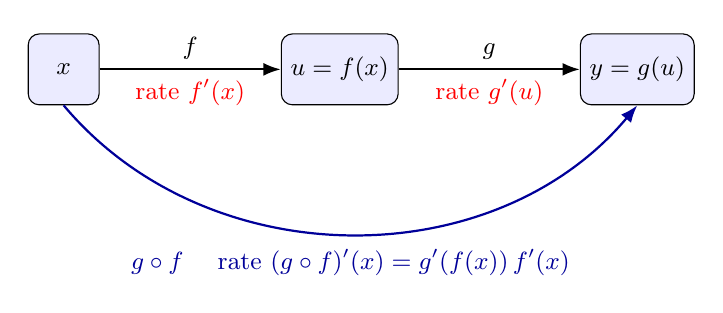
\begin{tikzpicture}[>={Latex[length=2.2mm]}, node distance=2.3cm, every node/.style={font=\small}]
	\node[draw, rounded corners, fill=blue!8, minimum size=9mm] (x) {$x$};
	\node[draw, rounded corners, fill=blue!8, minimum size=9mm, right=of x] (u) {$u=f(x)$};
	\node[draw, rounded corners, fill=blue!8, minimum size=9mm, right=of u] (y) {$y=g(u)$};
	\draw[->, thick] (x) -- node[above] {$f$} node[below, red] {rate $f'(x)$} (u);
	\draw[->, thick] (u) -- node[above] {$g$} node[below, red] {rate $g'(u)$} (y);
	\draw[->, thick, blue!60!black] (x.south) to[out=-50, in=-130] node[below, pos=0.5, yshift=-2pt] {$g\circ f$ \quad rate $(g\circ f)'(x)=g'(f(x))\,f'(x)$} (y.south);
\end{tikzpicture}
\end{document}
